\clearpage
\section{Signal Start Detection}
\label{sec:04_signalStartDetection}

\todo[inline]{This section seems a bit misplaced. I feel like "Team Evaluation"
should be the last evaluation section. Is there a reason why you can't put this
before that?}

In previous chapters, the importance of the signal start was emphasized.
% Due to the fact that the direction detection methods is
% executed on smaller frames than the actual whistle detection.
% To demonstrate this for the phase method, the frame to investigate is
% shifted with time \cref{subsec:04_frameNumber}.
Especially the result in \cref{subsec:03_phase} has shown that in fact, the
accuracy of the direction predictor decreases when evaluated on later samples
of the whistle signal.\todo{Maybe interpret this somewhere: give a reason
why shit makes sense (e.g. maybe because more reflections of the signal will
have reached the microphone)}
Also according to the outcome of \cref{subsec:04_psnr}, the \ac{GCC}
method performs best with frames near to the signal start. \todo[inline]{Get
rid of some cross-references and/or write more about what happened in these
chapters. (I don't remember what happened in 3.4 and 4.2.3 and jumping back and
forth is annoying.)}

% There are some reasons why other methods were tested to find the signal start.
In order to find a good solution for a highly reliable, accurate but
computationally tractable start detection, different approaches were
tested profoundly.
For high temporal\todo{I added "temporal" here because otherwise it seems unintuitive
that a less samples is better (because at the same time it might be harder to
predict from fewer samples as there is less information in the frame)} accuracy
either the number of samples in a frame have to be small\todo{Maybe rather say
that the frame as to be small? A low number of samples in a frame could also be
achieved by a smaller sampling rate, which would not help.} or the window must
be shifted with small steps which both implicit a large number of evaluations.
The existing whistle detection algorithm of the HULKs presented in
\cref{subsec:03_whistleDetection} is computationally intensive and has a low
accuracy for small frames\todo{Is "frames" actually the correct term (in
general)? Shouldn't it be "window"? I don't know what people use in signal
processing literature} as shown in \label{subsec:04_whistleDetection}.
Therefore, the goal is to identify a\todo{"looked" doesn't work this way. You are using this
quite a lot. Maybe grep the document for it and replace it.} simple algorithm for
the signal start detection. Ideally, this algorithm should be adaptable to
signals other than the whistle sounds.\todo{I would add a reference to the section
where you presented these algorithms. (this is only the evaluation, right?)}

Hereinafter, the performance of each method methods is evaluated by
analyzing the error between algorithmically determined start index
and manually labelled start index.
As a benchmark, the prediction accuracy is evaluated on 11 measurements on all
robots\todo{how many robots?} \todo{this sentence is missing some
words}\cref{subsec:04_labMeasurements}.
By the frame size of the \ac{FFT} being set to 256 samples for the
correlation methods, a start index error of at most 256 samples is
desired.
Therefore, a start index detection result is regarded as failure for errors
larger than 256 for the following sections.
Two metrics are specified to express the degree of failure.
The former counts the number of large errors for each channel.
In this case, 220 sample data for 11 measurements on five robots with
four channels each exist.\todo{I don't understand this sentence.}
The second metric reports the number of measurements for which any of the
channels failed. For this case, 55 measurements are given.\todo{Again, what is
this sentence saying? I thought we had 11 measurements? Or is it 11
measurements * 5 robots? Maybe simply write 55 in the first place (rather than
11)}.
% -----------------------------------------------------------------------------------------------------

\subsection{Whistle Detection}
\label{subsec:04_whistleDetection}

\todo[inline]{It is not immediately clear that with "whistle detection" you refer
to the "whistle detection of the HULKs", e.g. your "baseline"}
First, the accuracy of the whistle detection in regard of the start index
is evaluated.
Here, the start index is defined as the first index where the whistle detection
found a whistle.
With a frame size of 1024, the whistle detection algorithm fails in every of the
55 measurements with at least one channel if only an error of at most 256 samples
is permitted.
However, every error is in the range of 1024 samples which proves that the
approximate start of the whistle sound is detected correctly.
With a smaller frame size of 256, the temporal accuracy is improved but
introduces false positive detections.\todo{do you have numerical results here?}
With the results, one can say that the whistle detection is not sufficient
for the start detection or is at least not reliable as stand-alone solution.
Furthermore, this approach is limited to sounds in fixed and known frequency range.
%  failure rate of
% 9\si{\percent} in regard to every channel.
% In this work microphone data were saved as soon as the whistle detection module
% found a whistle sound in the audio samples.
% Due to this implementation, the algorithm does never fail to detect the whistle
% Standing alone, the error is always in the range of \si{\pm1024} samples due to the
% set frame size of 1024 samples.
% With a smaller frame size of 256, the accuracy gets better with an error of
% 9\si{\percent} in regard to the 220 sample data but has an error rate of
% 25,5\si{\percent} for the measurements.

% looking at the next 300
% values and with a step size of 50 the result is 15\si{\percent} and 36\si{\percent}
% and with step size 1, it is 13\si{\percent} and 33\si{\percent}.
% This is computationally very costly and the reward is small.

\subsection{ZCR}
\label{subsec:04_zcr}

For the evaluation of the \ac{ZCR},
the frame size is set to 256 samples and number of noise and signal frames
are set to 10 frames.
In 7\si{\percent} of the 220 channel sample data\todo{"sample data" sounds like
it is not a term. Maybe only "samples"?}, the method fails with a significant
error larger than 256 samples.\todo{I don't thing you have to repeat the 256
sample criterion every time. You defined what is considered a failure earlier.
Just say "failed".} In most cases, the method provides accurate results with
small error. Taking all measurements of robot 26 as example, the \ac{RMSE}
amounts 54.23 samples.\todo{Again, where is the data for this? Tables, figures?}

However, there are cases where the algorithm fails. Looking at those cases it
could be identified that the errors occur often due to incorrect assumptions
that the signal is present at the end of the buffered samples.
Some measurements prove that this is not always the case as shown in
\cref{fig:04_zcrFail}.
Here, the data of the front right channel of robot 21 with the whistle source
at position 5 in \cref{subsec:04_labMeasurements}
illustrates how the signal ended around 35000 samples already. \todo{Neither
the robot number, nor the position or the channel are relevant here I think.}
If the start index is determined at the point where the \ac{ZCR}
falls below the threshold searching backwards as stated in \cref{sec:02_signalStartDetection},
the detection fails.

In most cases, only one out of four channels produces a erroneous
result.\todo{Why? Doesn't the signal end early on all channels?}
Because the final start index on one robot is set equal for all channel,
the failure can be compensated with a simple voting procedure.
% -------------------------------------------------------------
\begin{figure}[ht]
	\centering
	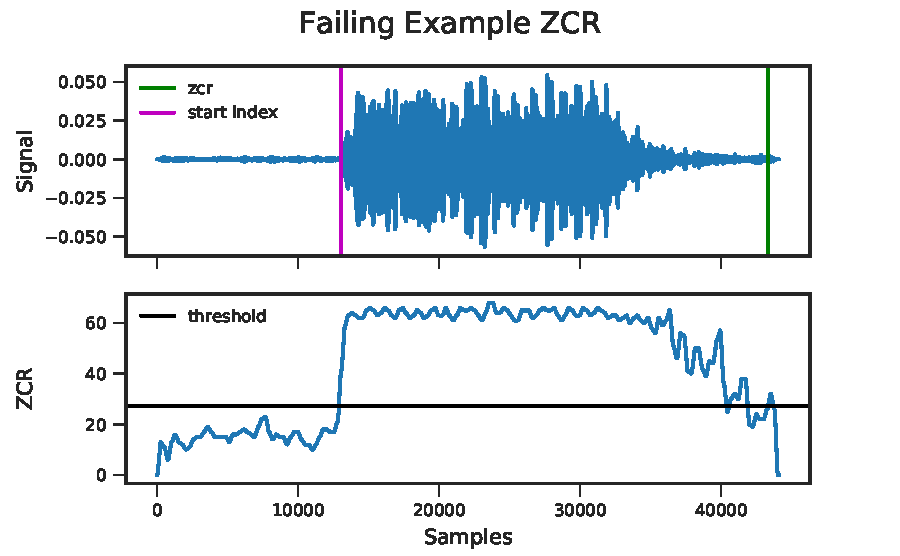
\includegraphics[]{figures/evaluation/zcr_fail}
	\caption{Channel 3 data from measurement 5 of \cref{subsec:04_labMeasurements}
		for robot number 21. A failing example for the start detection by \ac{ZCR}
		is shown.}
	\label{fig:04_zcrFail}
\end{figure}
% -------------------------------------------------------------
If the start index is determined at the point where the \ac{ZCR}
falls below the threshold searching backwards as stated in \cref{sec:02_signalStartDetection},
the detection fails.

In most cases, only one channel of four output a erroneous result.
Because the final start index on one robot is set equal for all channel,
the failure can be compensated with a smart voting procedure.

Another option exists by changing the process of finding the
threshold excess onwards.\todo{I don't understand what this is saying.}
In this case, the threshold is scaled with a factor of 1.25.
Results by this were poorer than the initially implemented manner
with a failure rate of 15\si{\percent}.\todo{Did you ever report the previous failure rate?}
By adding the constraint that multiple samples must exceed the
threshold successively, result can be slightly improved for the cost of higher
computational effort.

It should be noted that the poor performance of the \ac{ZCR} method with signal that
was cleaned with spectral subtraction previously. This surprising outcome is
convenient for the overall task, because the start index result can be embed
into the spectral subtraction, providing information for separating the noise
and signal part.\todo{I don't get what this paragraph is saying?}

\subsection{Entropy}
\label{subsec:04_entropy}

As discussed in \cref{subsec:02_Entropy} the entropy quantifies the amount
of chaos in a signal frame.\todo{Is this correct? Chaos is deterministic and not
the same as randomness}
Especially for signals to localize with unknown characteristics,
this method can be useful because no a-priori knowledge is needed.\todo{You should
probably say that the only prior knowledge must be, that the signal to detect
has lower entropy than the background noise.}
For all measurements this method yielded poorer results than the \ac{ZCR} method
with a failure rate of around 20\si{\percent}.
Best results are achieved with a frame size of 512 samples and a step size of 800
samples.
% \change[]{Explain what steps are? Maybe in implementation?}
However, for records with fading whistle the entropy method
generates more reliable results than the \ac{ZCR} method.\todo{What do you mean
by "fading whiste"? Whistles that don't have a distinct/abrupt start?}
Taking the same measurement as an example for which failure of the \ac{ZCR} method
was discussed earlier, \cref{fig:04_entropyGood} shows how the algorithm
detects the signal start correctly even though the whistle sound ended at
around 35000 samples. In this measurement, the start index errors of all four
channels were smaller than 40 samples.
% -------------------------------------------------------------
\begin{figure}[ht]
	\centering
	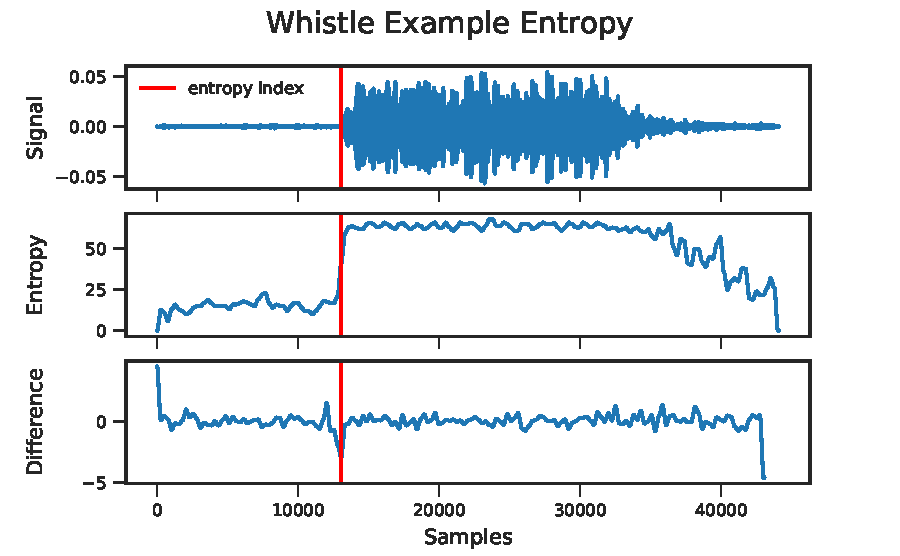
\includegraphics[]{figures/evaluation/entropy_good}
	\caption{Exemplary result of start index detection by entropy where
			the \ac{ZCR} method failed due to fading whistle
			at the data.}
	\label{fig:04_entropyGood}
\end{figure}
% -------------------------------------------------------------

% But as the entropy should be larger for noisy environment
% performance in other surrounding of measurement at \ac{RoboCup} is looked at.
% Entropy would be best for undefined signal -> distinguish between
% signal and noise without information
